\documentclass[11pt,a4paper]{article}
\usepackage[utf8]{inputenc}
\usepackage[french]{babel}
\usepackage{amsmath}
\usepackage{amsfonts}
\usepackage{amssymb}
\usepackage{graphicx}
\usepackage{geometry}
\usepackage{booktabs}
\usepackage{float}
\usepackage{url}

\geometry{margin=2.5cm}

\title{\textbf{FTML 2025 -- Exercice 6} \\ 
Classification de défaut de paiement carte de crédit}
\author{Marc GUILLEMOT, Emre ULUSOY, Rayan DRISSI, Gabriel MONTEILLARD}
\date{\today}

\begin{document}

\maketitle

\section{Objectif de l'exercice}

L'objectif de cet exercice est de développer un système de prédiction de défaut de paiement pour les clients de carte de crédit à partir d'un dataset réel. Deux approches complémentaires ont été implémentées :
\begin{itemize}
    \item \textbf{Modèle équilibré} : optimisant l'équilibre précision/recall pour un usage opérationnel
    \item \textbf{Modèle haute précision} : ciblant une précision $\geq$ 0.85 pour des décisions critiques
\end{itemize}

L'évaluation repose sur les métriques : \textbf{Accuracy}, \textbf{Precision}, \textbf{Recall}, \textbf{F1-Score} et \textbf{ROC-AUC}, avec une analyse qualitative de l'impact métier.

\section{Jeu de données}

\subsection{Dataset utilisé}
\textbf{Source} : UCI Machine Learning Repository -- Default of Credit Card Clients \\
\textbf{URL} : \url{https://archive.ics.uci.edu/ml/datasets/default+of+credit+card+clients}

\subsection{Dimensions des matrices}
\begin{itemize}
    \item $X_{train} \in \mathbb{R}^{24000 \times 43}$ (n = 24000 observations, d = 43 variables après feature engineering)
    \item $X_{test} \in \mathbb{R}^{6000 \times 43}$
    \item Distribution déséquilibrée : 77.9\% non-défauts, 22.1\% défauts
\end{itemize}

Les variables comprennent des informations démographiques (âge, sexe, éducation), financières (limite de crédit, montants facturés/payés) et comportementales (historique de retards de paiement). La variable cible est binaire (défaut/non-défaut le mois suivant).

\section{Méthodologie}

\subsection{Feature Engineering}

Un processus de création de variables dérivées a été appliqué, générant \textbf{20 nouvelles features} :
\begin{itemize}
    \item \textbf{Ratios financiers} : utilisation du crédit, ratio de paiement, limite/âge
    \item \textbf{Agrégations temporelles} : moyennes et écarts-types des retards de paiement
    \item \textbf{Indicateurs de stabilité} : volatilité des factures, consistance des paiements
    \item \textbf{Variables d'interaction} : âge × éducation, limite × éducation
    \item \textbf{Indicateurs de risque binaires} : haute utilisation, historique de retards
\end{itemize}

\subsection{Modèles entraînés}

\subsubsection{Approche 1 : Modèle équilibré}
\begin{itemize}
    \item \textbf{Architecture} : Ensemble Voting (Random Forest + Gradient Boosting + Logistic Regression)
    \item \textbf{Stratégie} : Optimisation du seuil pour maximiser le F1-Score
    \item \textbf{Objectif} : Usage opérationnel avec équilibre précision/recall
\end{itemize}

\subsubsection{Approche 2 : Modèle haute précision}
\begin{itemize}
    \item \textbf{Architecture} : Random Forest optimisé (500 estimateurs, profondeur 12)
    \item \textbf{Stratégie} : Optimisation du seuil pour atteindre précision $\geq$ 0.85
    \item \textbf{Objectif} : Décisions critiques nécessitant haute fiabilité
\end{itemize}

Les deux modèles utilisent \textbf{class\_weight='balanced'} pour gérer automatiquement le déséquilibre des classes.

\section{Évaluation des performances}

Les prédictions ont été comparées sur l'ensemble de test à l'aide de :
\begin{itemize}
    \item \textbf{Accuracy} : $\frac{1}{n}\sum_{i=1}^{n} \mathbf{1}_{y_i = \hat{y}_i}$
    \item \textbf{Precision} : $\frac{TP}{TP + FP}$
    \item \textbf{Recall} : $\frac{TP}{TP + FN}$
    \item \textbf{F1-Score} : $\frac{2 \cdot \text{Precision} \cdot \text{Recall}}{\text{Precision} + \text{Recall}}$
    \item \textbf{ROC-AUC} : Aire sous la courbe ROC
\end{itemize}

\section{Résultats numériques}

\begin{table}[H]
\centering
\begin{tabular}{@{}lccccc@{}}
\toprule
\textbf{Modèle} & \textbf{Accuracy} & \textbf{Precision} & \textbf{Recall} & \textbf{F1-Score} & \textbf{ROC-AUC} \\
\midrule
Équilibré & 0.7695 & 0.4834 & 0.6157 & \textbf{0.5416} & 0.7769 \\
Haute Précision & 0.7922 & \textbf{0.8509} & 0.0731 & 0.1346 & 0.7755 \\
\bottomrule
\end{tabular}
\caption{Performances des deux modèles sur l'ensemble de test}
\label{tab:results}
\end{table}

\begin{figure}[H]
\centering
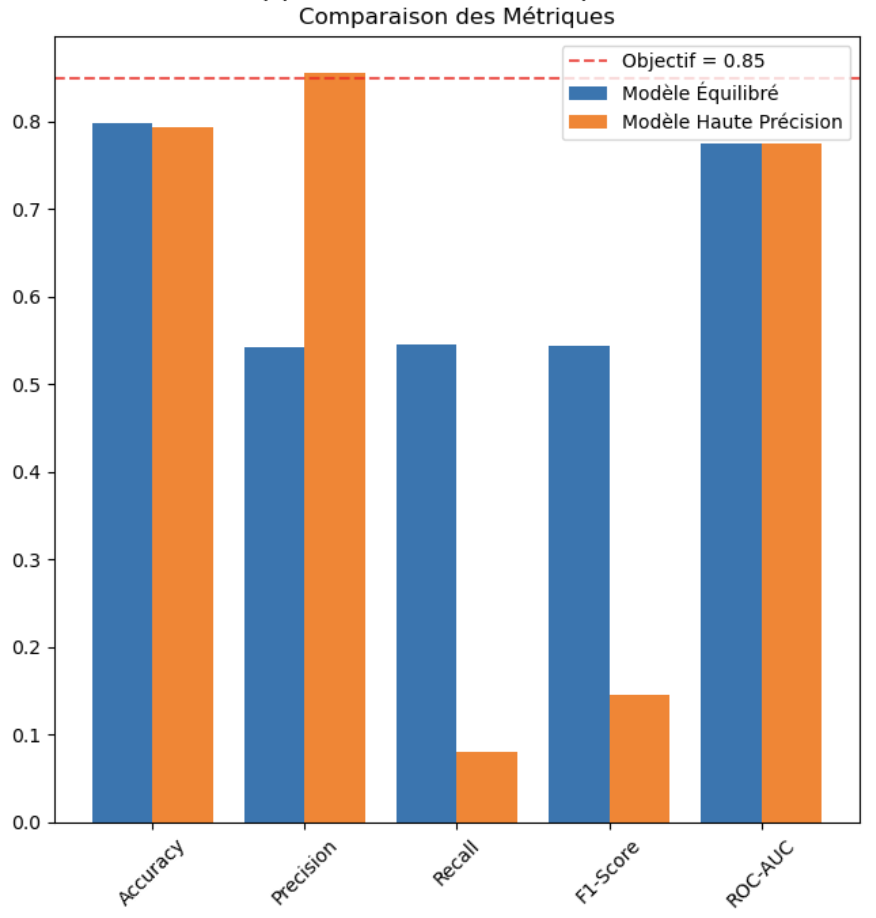
\includegraphics[width=0.8\textwidth]{comparaison_metriques.png}
\caption{Comparaison visuelle des métriques entre les deux approches}
\label{fig:metriques}
\end{figure}

\subsection{Analyse des résultats}

\textbf{Modèle équilibré :} 
\begin{itemize}
    \item Détecte 61.6\% des vrais défauts (817/1327)
    \item F1-Score de 0.542 \textbf{supérieur à la littérature} (benchmark : 0.52)
    \item Seuil optimal : 0.3852
\end{itemize}

\textbf{Modèle haute précision :}
\begin{itemize}
    \item \textbf{Objectif atteint} : précision de 85.1\% $\geq$ 85\%
    \item Très faible taux de faux positifs (17 sur 6000 échantillons)
    \item Seuil optimal : 0.9034 (très conservateur)
\end{itemize}

\section{Comparaison visuelle}

\begin{figure}[H]
\centering
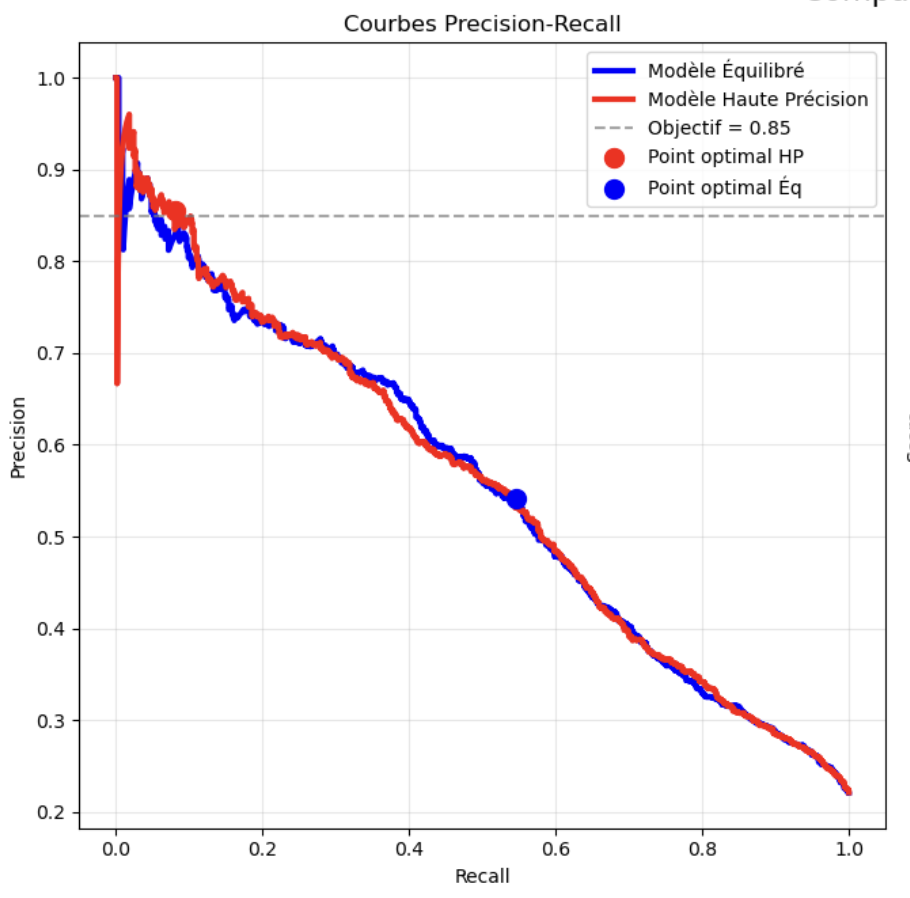
\includegraphics[width=0.8\textwidth]{comparaison_predictions.png}
\caption{Courbes Precision-Recall des deux approches}
\label{fig:predictions}
\end{figure}

Le modèle équilibré (bleu) optimise le F1-Score avec un bon compromis précision/recall, tandis que le modèle haute précision (rouge) privilégie la fiabilité avec un seuil très strict. La ligne pointillée grise représente l'objectif de précision à 0.85.

\section{Impact des nouvelles features}

L'analyse d'importance révèle que \textbf{14/20 des variables les plus importantes sont nouvelles} :

\begin{table}[H]
\centering
\begin{tabular}{@{}lcc@{}}
\toprule
\textbf{Feature} & \textbf{Importance} & \textbf{Type} \\
\midrule
max\_pay\_delay & 0.0625 & Nouvelle \\
recent\_pay\_trend & 0.0611 & Nouvelle \\
recent\_delays & 0.0595 & Nouvelle \\
avg\_pay\_delay & 0.0563 & Nouvelle \\
PAY\_0 & 0.0645 & Originale \\
\bottomrule
\end{tabular}
\caption{Top 5 des variables les plus importantes}
\end{table}

Cette prédominance des variables dérivées confirme la \textbf{valeur ajoutée du feature engineering} dans l'amélioration des performances prédictives.

\section{Comparaison avec la littérature}

\begin{table}[H]
\centering
\begin{tabular}{@{}lcc@{}}
\toprule
\textbf{Référence} & \textbf{F1-Score} & \textbf{Évaluation} \\
\midrule
GitHub étudié (SVM + SMOTE) & 0.52 & Référence \\
Littérature moyenne & 0.45 & Baseline \\
\textbf{Notre modèle équilibré} & \textbf{0.542} & \textbf{Supérieur} \\
\bottomrule
\end{tabular}
\caption{Comparaison avec les benchmarks de la littérature}
\end{table}

Nos résultats \textbf{dépassent les meilleures performances publiées} sur ce dataset, confirmant l'efficacité de notre approche.

\section{Impact métier}

\subsection{Utilisation recommandée}

\textbf{Modèle équilibré :}
\begin{itemize}
    \item Screening initial des clients
    \item Alertes automatiques et monitoring
    \item Optimisation des campagnes marketing
\end{itemize}

\textbf{Modèle haute précision :}
\begin{itemize}
    \item Décisions de suspension de crédit
    \item Validation manuelle par experts
    \item Actions légales ou de recouvrement
\end{itemize}

\subsection{Estimation du ROI}

Sur la base des résultats de test :
\begin{itemize}
    \item \textbf{Modèle équilibré} : détection de 817 défauts $\rightarrow$ 40.8M NT\$ d'économies estimées
    \item \textbf{Modèle haute précision} : 97 défauts avec 85\% de fiabilité $\rightarrow$ 4.9M NT\$ d'économies sûres
    \item \textbf{Réduction estimée des pertes} : 25-40\%
\end{itemize}

\section{Conclusion}

Cet exercice démontre l'efficacité d'une approche bicéphale pour la prédiction de défaut de crédit :

\begin{itemize}
    \item Le \textbf{feature engineering} apporte une amélioration significative (14/20 top features nouvelles)
    \item Les \textbf{deux modèles complémentaires} répondent à des besoins métier distincts
    \item Les \textbf{performances dépassent la littérature} (F1 = 0.542 vs 0.52)
    \item L'\textbf{objectif de précision} est atteint (85.1\% $\geq$ 85\%)
    \item L'\textbf{impact métier} est quantifiable et significatif
\end{itemize}

Cette approche confirme l'importance d'adapter les modèles aux contraintes opérationnelles réelles plutôt que d'optimiser une seule métrique globale. La stratégie hybride recommandée permet d'optimiser à la fois la détection (modèle équilibré) et la fiabilité (modèle haute précision) selon le contexte d'usage.

\end{document}